\documentclass[11pt,a4paper]{article}
\usepackage[T1]{fontenc}
\usepackage[margin=2.3cm]{geometry}
\usepackage{amsmath,amssymb}
\usepackage{graphicx}
\usepackage[dvipsnames]{xcolor}
\usepackage{enumitem}
\usepackage[colorlinks=true,linkcolor=blue,urlcolor=blue]{hyperref}
\setlength{\parskip}{0.6em}
\setlength{\parindent}{0pt}
\begin{document}

\begin{center}{\LARGE\bfseries openexoplanet}\\[0.4em]{\large Find a planet around another star from a tiny dip in its starlight, in three sessions.}\\[0.2em]\small PAN IIT OSS explainer \textbullet{} secondary school to diploma / undergraduate (levels 3-5)\end{center}

\section*{Why this exists}
Most known planets around other stars were found by watching starlight dip. This explainer shows the mathematics of that dip, from the area covered by a planet to a search through a noisy light curve, using only simple geometry and a little statistics.

\section*{The end goal}
Find a planet around another star from a dip in starlight. The end goal is to find a planet around another star from a dip in its starlight, as space telescopes do: clean the light curve, search it for a repeating dip, test whether it is a planet, and measure the planet's size and orbit.

\section*{How the three sessions build up}
\begin{enumerate}[nosep]
\item \textbf{Session 1: A planet in front of a star dims it} (Level 1, conceptual interactive model, 60 min).
\item \textbf{Session 2: The mathematics of a transit} (Level 2, mathematical engineering model, 75 min).
\item \textbf{Session 3: Find the planet in a noisy light curve} (Level 3, simulation and validation, 90 min).
\end{enumerate}

\section{Session 1: A planet in front of a star dims it}

\subsection*{A. Real-world problem}
Stars are so far away that even the best telescopes see them as single points of light, and a planet next to a star is lost in its glare. But if the planet's orbit is seen edge-on, the planet passes in front of its star once per orbit and blocks a little of the light. A telescope that measures the star's brightness again and again sees a tiny, regular dip. How deep is the dip, how often does it repeat, and how do you tell it from random noise?

\subsection*{B. Concept and theory}
A light curve is a graph of a star's brightness (1 = normal) against time. A transit is a dip that happens when a planet's dark disk covers part of the star's bright disk. The fraction of light blocked equals the fraction of the star's disk that is covered, which is the ratio of the two disk areas: (pi Rp\textasciicircum{}2) / (pi Rs\textasciicircum{}2) = (Rp/Rs)\textasciicircum{}2. The planet comes back once every orbit, so the gap between the centres of neighbouring dips is the orbital period P. Real measurements are noisy, so a point only counts as part of a dip if it lies below a threshold, and we require a few low points in a row.

\begin{itemize}[nosep]
\item Rp: planet radius (km (any length unit))
\item Rs: star radius (same unit as Rp)
\item k = Rp/Rs: radius ratio (no unit)
\item depth: fraction of starlight blocked (no unit (0.01 = 1 percent))
\item P: orbital period = time between dips (days)
\item t: time (days)
\end{itemize}

\begin{equation*}
\text{depth}=\frac{\pi R_p^2}{\pi R_s^2}=\left(\frac{R_p}{R_s}\right)^2=k^2
\end{equation*}

\begin{equation*}
t_n=t_0+nP\qquad\Rightarrow\qquad P=t_{n+1}-t_n
\end{equation*}

\begin{center}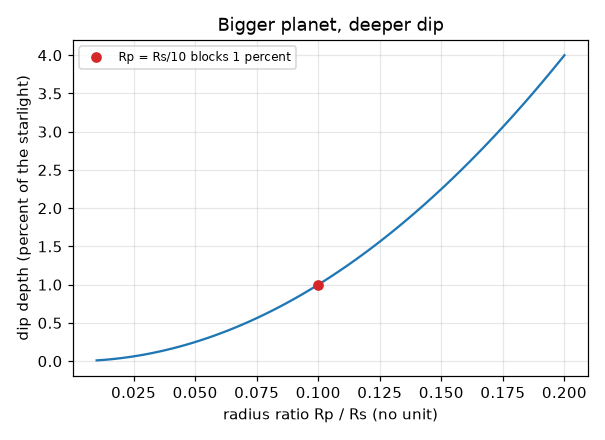
\includegraphics[width=0.85\linewidth]{figures/s01_depth_vs_size.png}\\\small Depth against radius ratio: a planet with a tenth of the star's radius blocks 1 percent.\end{center}

\subsection*{E. Worked example}
A star dips by 0.0025 (0.25 percent) with dip centres at days 2, 7 and 12. Find the orbital period and the planet-to-star radius ratio.
\begin{enumerate}[nosep]
\item Gaps between dip centres: 7 - 2 = 5 days and 12 - 7 = 5 days, so P = 5 days.
\item depth = k\textasciicircum{}2 = 0.0025, so k = sqrt(0.0025) = 0.05.
\item Check: a planet with 5 percent of the star's radius covers 0.05 x 0.05 = 0.0025 of its disk.
\end{enumerate}
\textbf{Answer.} Period 5 days; radius ratio Rp/Rs = 0.05.

\subsection*{F. Questions}
\begin{enumerate}[nosep]
\item \textbf{Conceptual.} Why does a transit only happen for some planets? Why do astronomers need to watch a star for longer than one orbit to be sure about a planet?
\item \textbf{Numerical.} A planet has half the radius of its star. What fraction of the light does it block? Is that realistic for a planet?
\item \textbf{Graph and simulation interpretation.} In the slider app the graph shows dips with period 3 days. You raise the period to 6 days but keep the planet size. What changes on the graph, and what stays the same?
\item \textbf{Design and optimisation challenge.} Design: you can watch a star for 12 days. A planet has a period of 5 days. What is the smallest number of dips you will see, and what is the longest period for which you are guaranteed to see two dips?
\end{enumerate}

\section{Session 2: The mathematics of a transit}

\subsection*{A. Real-world problem}
Jupiter blocks about 1 percent of the Sun's light and is easy to detect. Earth blocks less than one hundredth of that. Real stars are also not flat disks: they are dimmer at the edge. And the telescope's measurements are noisy. How much noise can we tolerate if we want to see an Earth-size planet around a Sun-like star in three transits?

\subsection*{B. Concept and theory}
The depth is k\textasciicircum{}2 where k = Rp/Rs. Put the star (radius 1) at the origin and the planet (radius k) at a distance z from its centre. For a flat star the flux is 1 minus the overlapping area of the two circles divided by the star's area pi. A real star is brighter at the centre; with mu = cos(angle to the line of sight) = sqrt(1 - r\textasciicircum{}2) at radius r on the disk, the quadratic law I(mu)/I(1) = 1 - u1 (1 - mu) - u2 (1 - mu)\textasciicircum{}2 describes the dimming towards the edge, with illustrative coefficients u1 = 0.40 and u2 = 0.25. The flux is 1 minus the light under the planet divided by the star's total light, found here on a fine grid. For a circular orbit of period P around a star of mass M, Kepler's third law gives the orbit radius a. The planet's distance from the star's centre in the sky is z = sqrt((a/Rs)\textasciicircum{}2 sin\textasciicircum{}2 phi + b\textasciicircum{}2 cos\textasciicircum{}2 phi), where b = (a/Rs) cos i is the impact parameter, and the transit lasts while z \textless{} 1 + k, giving T \textasciitilde{} (P/pi)(Rs/a) sqrt((1+k)\textasciicircum{}2 - b\textasciicircum{}2). Transit n happens at t0 + nP, so a straight-line fit of mid-times against n gives P. With n\_in measurements inside transits, each with noise sigma, the depth is measured to sigma / sqrt(n\_in), so SNR = depth sqrt(n\_in) / sigma.

\begin{itemize}[nosep]
\item k = Rp/Rs: radius ratio (no unit)
\item z: distance between planet and star centres, in star radii (no unit)
\item u1, u2: limb-darkening coefficients (0.40, 0.25 here) (no unit)
\item mu: cos of the angle between line of sight and the surface normal (no unit)
\item P: orbital period (days)
\item a: orbit radius (m)
\item G M: gravitational parameter of the star (1.327e20 for the Sun) (m\textasciicircum{}3 / s\textasciicircum{}2)
\item b: impact parameter: closest sky distance of the planet's path from the star's centre (star radii)
\item i: orbit inclination (90 degrees = edge-on) (degrees)
\item T: transit duration (first to last contact) (days or hours)
\item sigma: noise per measurement (fraction of the star's flux (1e-6 = 1 ppm))
\item n\_in: number of measurements inside transits (count)
\item SNR: signal-to-noise ratio (no unit)
\end{itemize}

\begin{equation*}
\delta=k^2=\left(\frac{R_p}{R_s}\right)^2
\end{equation*}

\begin{equation*}
\frac{I(\mu)}{I(1)}=1-u_1(1-\mu)-u_2(1-\mu)^2,\qquad \mu=\sqrt{1-r^2}
\end{equation*}

\begin{equation*}
F=1-\frac{\iint_{\text{planet}} I\,dA}{\iint_{\text{star}} I\,dA},\qquad \iint_{\text{star}} I\,dA=\pi\left(1-\frac{u_1}{3}-\frac{u_2}{6}\right)
\end{equation*}

\begin{equation*}
a=\left(\frac{GMP^2}{4\pi^2}\right)^{1/3}
\end{equation*}

\begin{equation*}
b=\frac{a}{R_s}\cos i,\qquad T\approx\frac{P}{\pi}\frac{R_s}{a}\sqrt{(1+k)^2-b^2}
\end{equation*}

\begin{equation*}
\mathrm{SNR}=\frac{\delta\sqrt{n_{\rm in}}}{\sigma}\;\Rightarrow\;\sigma_{\max}=\frac{\delta\sqrt{n_{\rm in}}}{\mathrm{SNR}}
\end{equation*}

\begin{center}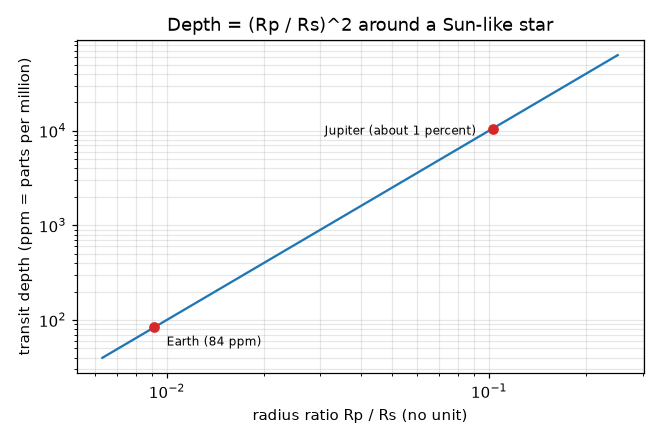
\includegraphics[width=0.85\linewidth]{figures/s02_depth_vs_radius.png}\\\small Depth against radius ratio on log axes, with Jupiter and Earth marked.\end{center}

\subsection*{E. Worked example}
An Earth twin crosses the centre of the Sun (b = 0) once per 365.25 days. Find its depth, a/Rs, the transit duration, and the noise per 30-minute measurement needed to detect it at SNR 7 from 3 transits.
\begin{enumerate}[nosep]
\item k = 6371 / 695700 = 0.009158 and depth = k\textasciicircum{}2 = 8.39e-5 = 83.9 ppm.
\item Kepler: a = (GM P\textasciicircum{}2 / 4 pi\textasciicircum{}2)\textasciicircum{}(1/3) = 1.496e11 m, which is 149.6 million km and a/Rs = 215.0.
\item T = (P/pi)(Rs/a) sqrt((1+k)\textasciicircum{}2) = (365.25/3.1416)(1/215.0)(1.00916) = 0.546 days = 13.10 hours.
\item A 30-minute cadence gives floor(13.10 / 0.5) = 26 measurements per transit, so n\_in = 3 x 26 = 78.
\item sigma\_max = depth x sqrt(n\_in) / SNR = 83.9 ppm x sqrt(78) / 7 = 105.8 ppm per measurement.
\item Check by simulation: the mean of 78 points with 105.8 ppm noise scatters by 105.8/sqrt(78) = 12.0 ppm, and 83.9/12.15 = 6.9, close to 7.
\end{enumerate}
\textbf{Answer.} Depth 83.9 ppm, a/Rs = 215.0, duration 13.10 hours, 26 points per transit; the noise must be below about 106 ppm per 30-minute point.

\subsection*{F. Questions}
\begin{enumerate}[nosep]
\item \textbf{Conceptual.} Why is the limb-darkened transit deeper in the middle than (Rp/Rs)\textasciicircum{}2, and why are its edges rounder?
\item \textbf{Numerical.} A planet with a radius of 2 Earth radii orbits a star of 0.5 solar radii. Find the transit depth in ppm.
\item \textbf{Graph and simulation interpretation.} In the duration-against-b graph (k = 0.1, P = 3 d), read the duration at b = 0 and at b = 0.8. Why is it shorter at b = 0.8?
\item \textbf{Design and optimisation challenge.} Design: your telescope gives 200 ppm noise per 30-minute point. How many transits of an Earth twin around a Sun-like star do you need for SNR 7? Is that practical?
\end{enumerate}

\section{Session 3: Find the planet in a noisy light curve}

\subsection*{A. Real-world problem}
A real light curve is not a clean box: the star's own brightness drifts as spots rotate in and out of view, the noise can be larger than the dip in a single measurement, and the telescope sometimes stops looking. How do you find a regular dip of half a percent inside that? And once you find one, how do you know it is a planet and not a fluke of the noise or a second star eclipsing the first?

\subsection*{B. Concept and theory}
Step 1, detrend: divide the light curve by a moving median (the median of all points within a window). The slow variability survives in the median and is removed by the division. If the window is shorter than about three transit durations, the median follows the transit itself and the division erases it. Step 2, search: fold the data on a trial period; if the period is right the transits stack and a box-shaped dip appears. Box Least Squares scans trial periods, box durations and start phases, and for each box computes SNR = (mean outside - mean inside) / (sigma sqrt(1/n\_in + 1/n\_out)). The period with the largest SNR is the candidate. Folding at half the period leaves half the folded dips empty, and folding at twice the period shows each transit only once per fold, so both give a weaker peak at P/2 and 2P: aliases. Step 3, vet: an eclipsing binary has a deeper primary and shallower secondary eclipse; BLS may lock on half its orbit, so odd and even events have different depths. A planet gives equal depths. Step 4, false alarms: run the same search on pure noise many times, and record the largest SNR each time. The fraction of runs that beat a threshold is the false-alarm rate.

\begin{itemize}[nosep]
\item t: time (days)
\item f: relative flux (1 = normal) (no unit)
\item window: width of the moving median (days)
\item P: trial or true period (days)
\item t0: mid-transit time (days)
\item n\_in, n\_out: number of points inside and outside the box (count)
\item sigma: noise per point (fraction of flux)
\item SNR: signal-to-noise ratio of the box (no unit)
\item k: radius ratio (no unit)
\end{itemize}

\begin{equation*}
f_{\rm flat}(t)=\frac{f(t)}{\mathrm{median}\{f(t'):|t'-t|<w/2\}}
\end{equation*}

\begin{equation*}
\mathrm{SNR}(P,t_0,d)=\frac{\bar f_{\rm out}-\bar f_{\rm in}}{\sigma\sqrt{1/n_{\rm in}+1/n_{\rm out}}}
\end{equation*}

\begin{equation*}
k\approx\sqrt{\delta},\qquad R_p=k\,R_s\;\left(\frac{695700}{6371}\ \text{Earth radii per solar radius}\right)
\end{equation*}

\begin{center}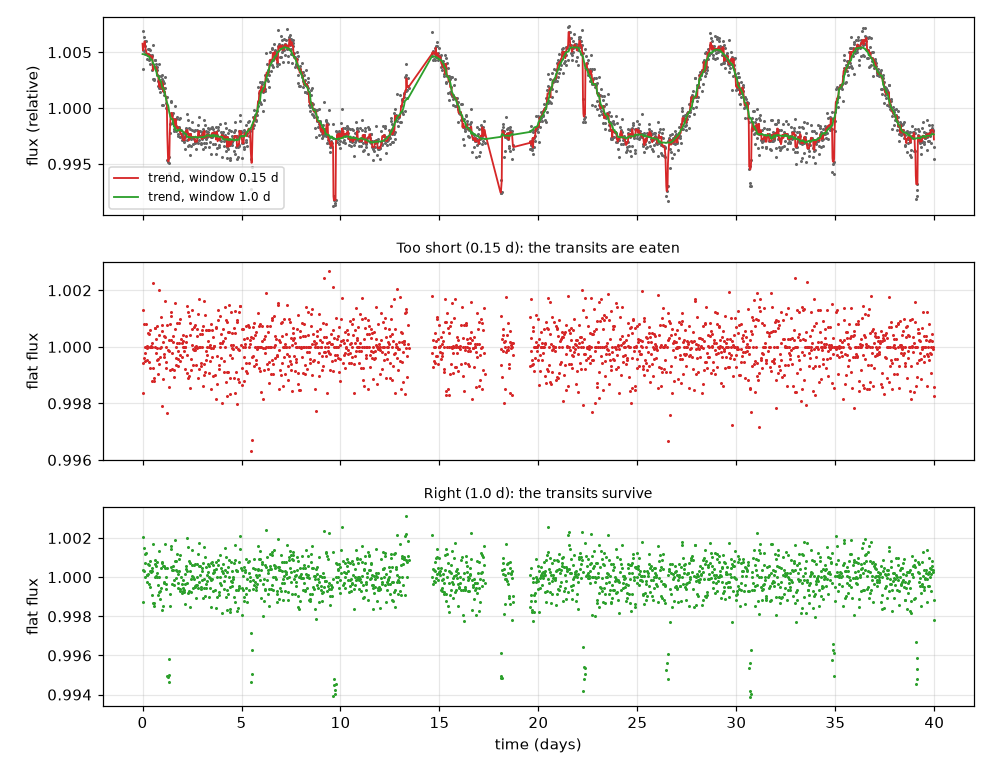
\includegraphics[width=0.85\linewidth]{figures/s03_detrend_windows.png}\\\small Raw light curve with a too-short (red) and a good (green) moving median; the short window erases the transits.\end{center}

\subsection*{E. Worked example}
Use the mini-project light curve (star of assumed radius 0.9 solar radii, 50 days). Find the first planet and report its period, depth, radius ratio and radius in Earth radii, with the odd-even check.
\begin{enumerate}[nosep]
\item Detrend with a 1.0 day moving median, then run BLS and refine: the strongest peak is at P = 6.431 days with SNR 25.
\item The box depth is 2311 ppm (0.002311).
\item Radius ratio: k = sqrt(0.002311) = 0.0481.
\item Radius: 0.0481 x 0.9 x 695700 / 6371 = 4.73, so about 4.7 Earth radii (the injected planet has 4.9).
\item Odd-even: the depths of odd and even transits differ by only 0.5 sigma, below 3 sigma, so the candidate passes.
\item Mask the transits and search again: the second planet appears at P = 2.710 days with SNR 9.5, radius 2.6 Earth radii, odd-even 1.7 sigma. Both are above the SNR threshold of 7.
\end{enumerate}
\textbf{Answer.} Planet 1: P = 6.431 d, depth 2311 ppm, k = 0.048, about 4.7 Earth radii. Planet 2: P = 2.710 d, about 2.6 Earth radii. Both pass the odd-even check.

\subsection*{F. Questions}
\begin{enumerate}[nosep]
\item \textbf{Conceptual.} Why can BLS not tell the difference between period P and period 2P if every second transit falls in a data gap? What would you need to resolve it?
\item \textbf{Numerical.} A candidate has depth 0.0025 around a star of radius 0.9 solar radii. Find the planet radius in Earth radii.
\item \textbf{Graph and simulation interpretation.} In the periodogram of the 4.2 day planet, which peaks are at about 2.1 and 8.4 days, and how do their heights compare with the main peak? Why are they lower?
\item \textbf{Design and optimisation challenge.} Design: the transit lasts 0.12 days and the star's brightness varies with a period of 7.3 days. Choose a moving-median window and say what limits it on each side. Then say which SNR threshold you would adopt for a search like the one in the lesson and why.
\end{enumerate}

\section{Real-world mini-project}
\textbf{Find the planets in a provided light curve.} A telescope watched one star for 50 days at 30-minute cadence. The star has spots that dim it by a few tenths of a percent as it rotates, there are gaps in the data, and two planets are hiding in it. \texttt{project\_lightcurve()} from Session 3 returns the data. Assume the star has radius 0.9 solar radii. Find both planets one after the other: detrend with a 1 day moving median, run BLS, refine, vet with the odd-even check, mask the transits you found, and search again.

\section{The path ahead}
\begin{enumerate}[nosep]
\item \textbf{Session 4: A detrend that cannot eat the transit.} A detrending routine that finds a candidate, masks its transits and refits the trend.
\item \textbf{Session 5: Fit the transit with limb darkening.} A fitting function that returns the radius ratio and impact parameter with uncertainties.
\item \textbf{Session 6: A weaker planet.} A search that detects a 600 ppm planet (period 4.2 days) at the same noise as the demo.
\item \textbf{Session 7: Unmask the binary.} A vetting function that tests the folded curve at phase 0.5 and at twice the BLS period.
\item \textbf{Session 8: Real data.} The full pipeline run on a downloaded real light curve of a known planet.
\end{enumerate}

\section{Answers and hints}

\subsection*{Session 1}
\begin{enumerate}[nosep]
\item \textbf{Conceptual.} Hint: Think about the orbit's tilt, and about what one dip alone can and cannot tell you. Solution: A transit needs the orbit to be seen almost edge-on; for most orbits the planet passes above or below the star and nothing dips. One dip could be a glitch, a flare, a spot or noise; two or more dips with the same depth and equal spacing give a period and strong evidence that a planet repeats its pass.
\item \textbf{Numerical.} Hint: depth = k\textasciicircum{}2 with k = 0.5. Solution: depth = 0.5\textasciicircum{}2 = 0.25, so 25 percent of the light. That is far larger than any real planet around a Sun-like star: even Jupiter blocks only about 1 percent. A dip that deep would more likely be a second star (a binary).
\item \textbf{Graph and simulation interpretation.} Hint: Compare the depth and the spacing of the dips. Solution: The dips become twice as far apart (6 days) and fewer fit in 12 days (two instead of four); their depth does not change because the planet size did not change. Depth depends on k only; spacing depends on P only.
\item \textbf{Design and optimisation challenge.} Hint: Dips are spaced P apart. Slide the first dip anywhere in the first P days. Solution: With P = 5 days in 12 days you see at least 2 dips (and up to 3, depending on where the first falls). To be sure of two dips, the 12-day run must contain two dips wherever the first falls: the first dip can occur as late as day P, and the second at day 2P, so we need 2P \textless{}= 12, i.e. P \textless{}= 6 days. Longer periods may show only one dip. Trade-off: watching longer finds longer periods.
\end{enumerate}

\subsection*{Session 2}
\begin{enumerate}[nosep]
\item \textbf{Conceptual.} Hint: Where on the star is the planet when it is in the middle, and how bright is that part compared with the average? Solution: At mid-transit (b = 0) the planet covers the centre, which is brighter than the star's average (the edge is dimmer), so it blocks more than its share of area: depth is about k\textasciicircum{}2 / (1 - u1/3 - u2/6) = 0.0121 for k = 0.1. At ingress and egress it covers the dim edge, which blocks less light, so the curve slopes gently.
\item \textbf{Numerical.} Hint: k = Rp / Rs with both radii in km. Solution: Rp = 2 x 6371 = 12742 km and Rs = 0.5 x 695700 = 347850 km, so k = 0.03663 and depth = k\textasciicircum{}2 = 1.342e-3 = 1342 ppm. Sanity check: smaller stars make the same planet look bigger; depth is much more than the 84 ppm of Earth around the Sun.
\item \textbf{Graph and simulation interpretation.} Hint: Use T = (P/pi)(Rs/a) sqrt((1+k)\textasciicircum{}2 - b\textasciicircum{}2) with a/Rs = 8.75. Solution: At b = 0: 2.88 hours; at b = 0.8: 1.98 hours. A path that crosses the star away from the centre is a shorter chord, so the planet is in front of the disk for less time; at b = 1 + k = 1.1 the path just misses and the duration is zero.
\item \textbf{Design and optimisation challenge.} Hint: n\_in = (SNR sigma / depth)\textasciicircum{}2, then divide by 26 points per transit and round up. Solution: n\_in = (7 x 200 / 83.9)\textasciicircum{}2 = 279 points, which is 279 / 26 = 10.7, so 11 transits. One transit a year means 11 years of observation, which is not practical for a single mission, so instead survey many stars, use a quieter telescope, or look at smaller stars where the depth is larger (see question B). Trade-off: noise, number of transits, and star size.
\end{enumerate}

\subsection*{Session 3}
\begin{enumerate}[nosep]
\item \textbf{Conceptual.} Hint: Which transits are actually in the data, and what does folding at P and at 2P do with them? Solution: If only the even transits are observed, folding at P and at 2P both stack the same set of transits and leave the same gaps, so the SNR is equal (28.2 and 28.1 in the lesson). Only data that include the missing transits (more observing time, or a second telescope) can show that there are also dips at the odd times.
\item \textbf{Numerical.} Hint: k = sqrt(depth); then Rp = k Rs x 695700 / 6371. Solution: k = sqrt(0.0025) = 0.05; Rp = 0.05 x 0.9 x 695700 / 6371 = 4.91 Earth radii. Units: solar radii converted with 695700 km / 6371 km = 109.2 Earth radii per solar radius. Sanity check: between Neptune and Saturn sizes is plausible for a 0.25 percent dip.
\item \textbf{Graph and simulation interpretation.} Hint: Think about what folding at half and at double the period does to the transits. Solution: They are the aliases at P/2 and 2P, with SNR of about 26 and 27 compared with 37 for the true period (both below 0.8 of the main peak). At P/2 only half of the folded cycles contain a transit, so the stacked dip is diluted; at 2P each transit is seen once per fold and only half the data contribute to the dip, so its SNR is smaller by about sqrt(2).
\item \textbf{Design and optimisation challenge.} Hint: Window at least 3 transit durations; not so long that the median cannot follow the variability. In 100 pure-noise runs, what was the largest SNR? Solution: The window must be at least 3 x 0.12 = 0.36 days or the median follows the transit (0.15 days keeps only 3 percent of the depth); it must be much shorter than 7.3 days or the median cannot follow the spots. 1.0 day keeps 94 percent of the depth. Pure noise gave at most SNR 5.2 in 100 runs and 7 percent of runs passed SNR 5, none passed SNR 6. A threshold of 7 is safe for this search (and is the value used by surveys), at the price of missing planets weaker than SNR 7. Trade-off: lower threshold finds more planets but more false alarms.
\end{enumerate}

\section{How to join}
Read \texttt{CONTRIBUTING.md} in the repository, then pick an issue labelled \texttt{good first issue}. Repository: \url{https://github.com/KrunalPanchal1995/openexoplanet}

\end{document}
